\documentclass[10pt, journal]{IEEEtran}

\usepackage[T1]{fontenc} % optional
\usepackage{cite}
\usepackage{url}
\usepackage{listings}
\usepackage[usenames]{xcolor}
\usepackage{fancyvrb}
\usepackage{graphicx}

\begin{document}
\title{Economies at a Glance - A Visualisation System}
\author{
\IEEEauthorblockN{Aden Kenny - 300334300}
}
\maketitle

\section{Introduction}
~\\
For the SWEN 422 course we were given a project to develop an information visualisation system. We were given relatively free rein over the dataset we chose, so long as it was related to one of the UN Millennium Sustainable Development Goals \cite{devgoals}. We chose the development goal of "Decent Work and Economic Growth" \cite{dec}. 

This goal relates to the health of the global economy and its ability to provide enough well paying jobs for everyone that wants to work. Therefore we decided to create an information visualisation system that allows anyone to gain a basic understanding of the health of the economy of any country, and how "good" the job opportunities in that country are.



\section{System Design and Justification}

Our dataset was scraped from the CIA World Factbook \cite{cia}, and the data provides an overall view of the economies of all the countries around the world, and various economic indicators. We chose this dataset as it allows the comparison of economies as a whole, which we considered to be the best proxy for overall "goodness" of work.

The dataset was downloaded as JSON and then the relevant information was extracted and cleaned up with a Python script. This allowed us to reduce the dataset size from 13.7MB to 220KB, mainly by removing data that was not relevant to our chosen development goal.

The system was created using TypeScript \cite{ts}, React \cite{react}, and D3.js \cite{d3}. This is a fairly standard combination for web development of visualisation systems, and this stack provided a nice blend of features, and ease of use. The system was designed to be a visualisation system and it was decided that a world map or chloropleth would be the main visualisation technique used by this project. DataMaps \cite{dms}, a D3.js library was chosen to provide the chloropleth.

The system, at a high level, consists of two main parts, the "data scraper" and the "visualisation system". The data scraper is a Python script that takes a JSON that consists of data scraped from the CIA World Factbook \cite{cia}. The script then cleans this data by removing parts of the data that are irrelevant to the system, i.e. non-economic data. The overall purpose of this part of the system was to prepare the data for the main part of the system, the visualisation system. The data was then stored in a Firebase \cite{firebase} database where it was queried by the visualisation system when needed. This provided a fairly simple separation of concerns between the data and the visualisation system.

The visualisation system formed the bulk of the project, with the majority of time and resources over the course of the project being spent on it. The visualisation system itself consisted of two main parts, the first being the previously mentioned world map (or chloropleth) view, and the second being a "graph view", that was based around a bar graph. 

Both views have a navigation bar at the top of the screen which allows the user to switch between views, switch the selected economic indicator, and to show a help menu. This navigation bar stays at the top of the application as we felt that it is always useful to the user.

\subsection{Map View}

It was decided that the map view would be the main screen, the screen that a user would first see when they used the system. This was decided because the world map gives a good overview of the data, and is a good starting place for a user to view the information that the system presents and therefore is built around. The user can zoom in and out, and pan the map using the control panel to the left of the world map.

The world map view has, as the name suggests, a world map at the centre of it. The countries on the world map are coloured in relation to their selected indicator value. This provides a colour gradient based on the indicators, and there are seven possible colours that a country can be shaded. The colours range from light yellow to brown. In order to get values for the shading, the range between the minimum and maximum values is calculated and then the range is split into seven equal parts. Each country, based on the selected indicator value, is then assigned a colour from the range. This colouring allows a user to quickly view the world map and gain a basic overview of the countries based on the selected indicator. This ability to quickly glance at an economy was a key goal that occurred frequently in our scenarios \cite{scenarios}. This meant that we placed a significant amount of emphasis on the importance of the map view, and resources were allocated as such.

The world map view also presents the advantage of being able to clearly communicate the relationship between countries based on economic indicators. This is especially apparent when countries fall into the same indicator range (one of the seven splits). In this case the countries will be shaded with the same colour and a relationship is strongly suggested. The shown relationships are also dynamic due to the ability of the user to change the economic indicator that is being displayed.

If a user wants to view more in depth information about a country, they can click on the country on the map and a panel is brought up to the right of the map. This panel lists all available economic indicators, not just the selected indicator. This allows the user to gain a detailed view of an individual economy, and it was a major goal that was listed in our scenarios \cite{scenarios}. The alternative to the design decision of having all the indicators shown in the side menu would be to have only the currently displayed indicator on the side menu. This has two major downsides, firstly, this would mean that the system would not display an overall view of an economy at all. Secondly, the alternative is partially fulfilled in the graph view portion of the software.

\subsection{Graph View}

The second main view is the graph view. It is designed for a more in depth comparison of indicators across countries. The map view has some weaknesses when showing indicators that have data points that are major outliers, as many countries will be the exact same shade, which makes drawing any conclusions from the visualisation difficult. The graph view is designed to help to mitigate this issue. Some indicators that are available in the map view are not available in the graph view as they do not make sense shown in a bar graph style. Examples of this include indicators based on rank (e.g. Venezuela having the lowest 223th lowest growth rate in 2017), as it makes little sense to plot this on a bar graph. 

The graph view has a side panel to the right. This panel includes the country select menu. This menu allows a user to select countries that they want to be displayed on the graph. The countries are, in the default view, grouped by region, and the user can click on any of the regions and each country in the region will be selected to be shown on the graph. The region groups can also be expanded so the user can select individual countries. Additionally, there is a search bar, and this means that the user can search specific countries individually to add to the comparison list. A user can add any number of countries to the comparison list, but adding 150 countries will probably diminish the usefulness of the graph, as would adding just one.

Once the user has selected a set of countries to show on the graph they can select an indicator they wish to be graphed. A graph is then drawn from the data, from the selected set of countries, for the selected indicator. The bars on the graph can be hovered over, and it will pop up with the exact value for that country, which helps the user to get more exact data, rather than being constrained with the graph when it can be hard to get the exact value of the bar from the axis scale.


\begin{figure}[h]
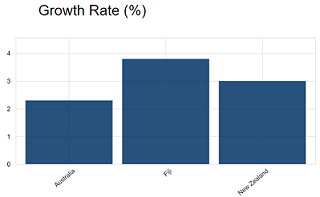
\includegraphics{graph.png}
\caption{A screenshot of the graph view showing growth rate versus country, with Australia, Fiji, and New Zealand being the selected countries}
\end{figure}


The graph view, as a whole, is more useful than the map view in some situations. It is especially useful if a user only wants to compare a small set of countries, such as a region. In this case using the map view would mean that a significant amount of irrelevant data (all the non-selected countries) would be presented to the user. However, if the user were to use the graph view, only information they have selected, which is hopefully relevant, will be shown to the user.

The graph view also helps our personas \cite{personas} complete their scenarios \cite{scenarios}, mainly scenarios where the persona wants to compare a region, or simply compare only a small number of countries as opposed to the world as a whole.

\subsection{Help Menu}

The help menu is a menu that can open from the navigation bar, which means that it is accessible in both the graph view and the map view. When the help button, which is on the navigation bar, is clicked the help "slideshow" pops up. This is a slideshow that opens on top of the currently selected view (either map or graph), it has three pages. Each of these pages is a help screen for a unique part of the system. The first help screen deals with the system as a whole, including introducing the system. The second and third screens provide help and tips for the map and graph view respectively.

\subsection{Comparison to Goals}

The goals of the Economies at a Glance project were listed in the Goals document \cite{goals} submitted as part of the group submission for this assignment, and they are as follows;

\begin{enumerate}
\item{Compare the economies of multiple countries}
\item{Gain an overall view of the global economy}
\item{Get in depth data on the economy of a country}
\item{Compare the economies of multiple countries in a region}
\end{enumerate}

I feel that all four of the listed goals have been met by the system that has been developed.

The first goal "Compare the economies of multiple countries", is met by both the map and the graph view, but they provide different ways of completing the goal.  The map view allows the user to compare economies by grouping similarly coloured countries (by the selected indicator). This is a less detailed and accurate comparison, but it can be done extremely quickly, and is a very good starting point, especially when comparing countries where there is a large range in values. The graph view allows the user to complete this goal by letting the user select the countries they wish to compare. This means that there is less irrelevant data or noise. It does mean that the data requires more analysis, a user cannot glance at the data as quickly as they could using the map view. 

The second goal was to "Gain an overall view of the global economy". This goal is quite similar to the first goal, but does have some differences. This goal means that a user will be comparing every country in the world, rather than a set of countries that they have chosen. This means that only the map view fulfils this goal, as while it is technically possible to display all the countries in the world on the graph view, it is quite impractical. Overall, the map view fulfils this goal as it allows the user to quickly gain insight into various economic indicators that present an overall "big picture" of the global economy.

The third goal was to "Get in depth data on the economy of a country". This goal means that user must be able to get all the available economic data the system has on the a single selected country. The system fulfils this goal by having the side panel that shows all the data available for that country. This provides an in depth view of the economy of the selected country as it displays all of the data that our system has on that specific country. 

The fourth goal was to "Compare the economies of multiple countries in a region". This goal was fulfilled by the graph view. This is because the graph view, while selecting countries, allows the user to easily select a whole region's worth of countries to be selected by clicking on the tickbox for that region. Once an indicator is selected, the graph will displayed with all the countries in the selected region(s). This view therefore shows indicators for all the countries in a region which means that this system goal is 
fulfilled by the graph view.

Overall, the system meets the set goals, and each of the two views play a part in meeting the goals, therefore I feel that all the major components of the system are well justified in their existence and design.

\section{Contributions}

In order to measure the contributions of each team, the system will be split into parts and a percentage of each part will be assigned to each group member based on work done on that specific component. There were four members in our group;

\begin{itemize}

\item{Aden Kenny - 300334300}
\item{Jeremy Purvis - 300334309}
\item{Ryan Zheng - 300334310}
\item{Simon Pope - 300334309}

\end{itemize}

~\\
The system will be split into seven parts;
\begin{itemize}
\item{Planning (Personas, Scenarios, Goals, Architecture)}
\item{Data set (Scraping, cleaning)}
\item{Map view}
\item{Graph view}
\item{Miscellaneous programming}
\item{Research (Libraries, Precedents)}
\item{Evaluation (Design, Implementation)}
\end{itemize}

\subsection{Planning (Personas, Scenarios, Goals, Architecture)}
\begin{itemize}

\item{Aden Kenny - 45\%}
\item{Jeremy Purvis - 5\%}
\item{Ryan Zheng - 5\%}
\item{Simon Pope - 45\%}

\end{itemize}

\subsection{Data Set (Scraping, Cleaning)}
\begin{itemize}

\item{Aden Kenny - 60\%}
\item{Jeremy Purvis - 0\%}
\item{Ryan Zheng - 0\%}
\item{Simon Pope - 40\%}

\end{itemize}

\subsection{Map View}
\begin{itemize}

\item{Aden Kenny - 45\%}
\item{Jeremy Purvis - 0\%}
\item{Ryan Zheng - 0\%}
\item{Simon Pope - 55\%}

\end{itemize}

\subsection{Graph View}
\begin{itemize}

\item{Aden Kenny - 8\%}
\item{Jeremy Purvis - 28.5\%}
\item{Ryan Zheng - 28.5\%}
\item{Simon Pope - 35\%}

\end{itemize}

\subsection{Miscellaneous Programming}
\begin{itemize}

\item{Aden Kenny - 27.5\%}
\item{Jeremy Purvis - 25\%}
\item{Ryan Zheng - 20\%}
\item{Simon Pope - 27.5\%}

\end{itemize}

\subsection{Research (Libraries, Precedents)}
\begin{itemize}

\item{Aden Kenny - 35\%}
\item{Jeremy Purvis - 20\%}
\item{Ryan Zheng - 15\%}
\item{Simon Pope - 30\%}

\end{itemize}

\subsection{Evaluation (Design, Implementation)}
\begin{itemize}

\item{Aden Kenny - 35\%}
\item{Jeremy Purvis - 0\%}
\item{Ryan Zheng - 0\%}
\item{Simon Pope - 65\%}

\end{itemize}


\subsection{Evaluation (Design, Implementation)}
\begin{itemize}

\item{Aden Kenny - 35\%}
\item{Jeremy Purvis - 0\%}
\item{Ryan Zheng - 0\%}
\item{Simon Pope - 65\%}

\end{itemize}



\subsection{Overall Contribution}

We can get a rough overall contribution by adding the percentages for each group member and then dividing that by the number of categories.
\begin{itemize}

\item{Aden Kenny - 37\%}
\item{Jeremy Purvis - 12\%}
\item{Ryan Zheng - 10\%}
\item{Simon Pope - 43\%}

~\\
Note that percentages do not add to 100\% due to rounding.

\end{itemize}



\section{Evaluation Description}

Our user study \cite{eval} was an online survey made with Google Forms \cite{forms}. It has three main sections, questions on the map view, questions on the graph view, and general questions about the system as a whole. As per the ethics approval, it was designed to be answered by 400-level ECS students, and therefore assumed some level of technological ability. The survey was posted on the SWEN 422 class Facebook page, and the 400-level Engineering page to find users who would participate.

It started with a standard disclaimer and had a required question where the user who was taking the survey had to agree to their survey responses being collected to continue. It then had three fairly simple questions where the user had to use the map view to get the answer. After this there were some questions asking the user about how they found the experience of using the map to find information, general feedback on the map, and some specific questions on the colouring scheme used.

The second part of the user study was a section where the user was asked questions that would be answered by using the graph view. The user would be asked a question such as "Which country has a higher portion of the workforce in services?" and given two choices. After these questions, there were a few questions on feedback for the graph page.

On the final page there was a question asking the user to rate the overall experience of the system on a scale of 1 to 5. There was also a final question that asked if the user had any further comments or general feedback on the system as a whole.

The questions therefore mainly consisted of two parts, firstly, feedback long answer questions that were designed to gauge the user's opinions on various features, and the system as a whole. There were also short answer questions that required the user to use the system to find the answers to simple questions. These questions were designed to test the effectiveness and ease of use of the system. If the system was ineffective or hard to use, the user would not be able to answer the question correctly.

\section{Evaluation Interpretation}

We had five responses to our user study which gives a sample size of n = 5. This, unfortunately is not a particularly large sample size, but conclusions can still be drawn from the results.

\subsection{Map View}

The first section of the user study focused on the map view. This was the area that we had spent the most time on, therefore we considered it to be the strong point of the system. There were three short answer questions in this section and two of them had a 100\% correct answer rate, and the third had an 80\% correct answer rate. This is a pretty good correct answer rate, and the one incorrect answer can be attributed to the shading system used for the map. This question asked users out of two countries, which country had a higher percentage of total wealth held by the 10\% of households. Unlike some other indicators that were used in the two previous questions, the colouring for this indicator has a lower percentage of wealth held by the top 10\% of households as a darker shade of brown. In some other indicators the higher value is shaded the more brown colours. This does show a flaw in the system, and it probably means that we should have been more careful when indicating that the indicators had flipped like they had for this indicator. Overall the map proved to be quite effective based on the short answer questions.

The next questions focused on long answer questions about the map. The users were also asked to rate the maps on a scale of 1 to 5 based on ease of use and other factors. The first question asked in the scale rating was "How difficult was it to find the information in the last section?".  1 on this scale was very hard, and 5 was very easy. This question had an average answer of 4, showing that, on the whole, users found the map fairly easy, but not perfectly easy, to use. 

The second question asked how the user rated the colouring system, with 1 being very bad and 5 being very good. The average answer was 3.4. This showed that the colouring system was viewed slightly positively. A possible hypothesis for this low rating is the confusion that the previously mentioned reverse colouring system may have inspired.

The third and final scale question asked users how useful they found the colour legend. As per the other questions, 1 represented very unhelpful, and 5 represented very helpful. The average answer for this question was 3. This was the lowest answer out of the three questions asked in this section, and this shows that users found the colour legend the least useful part of the map view. A possible hypothesis for this is that the users mainly relied on the shading of the map, and focused more on the relationships between the shades, rather than what the shades actually meant in terms of value.

We then had long answer questions which asked the users a few questions about the map. The first question asked users how they felt about the reversed colour gradient for some indicators. It was roughly split evenly between users saying it was useful, and that it was useful, but confusing and could probably do with some more explanation or explicit pointing out of it. 

The second long answer question asked users what aspects of the map they found useful. Two responses talked about finding the tooltip that appeared when hovering over countries as useful and a good feature. They liked the fact that it provided instant feedback, and was good for finding specific data values. Another user stated that they found the zoom tools useful, especially the reset zoom button after zooming in to look at a country. Another user stated that they found having all the countries displayed all together on the map as useful, as it provided a good "rough sense" of comparison.

The third long answer question asked users which aspects of the map could do with improvement. Users stated that map movement (rather than the zoom) felt a little unintuitive (map movement used arrow buttons rather than panning). A user stated that the map view is not very useful when the user does not know where a country is on the map. Another user stated that the data scale could potentially use some improvement. They felt that with some indicators, splitting the data into sevenths left only a few colours being used at once. They stated that a log scale could be useful in these cases. A user stated that, for the questions that the user study asked, the colouring was not particularly useful, they had to find specific values and that the colouring was not useful in this case.

Overall the users found the map to be fairly useful and easy to use, but did list some problems that were very valid and would be prime candidates for a fix in future versions of the system.

\subsection{Graph View}

The second page asked the user to use the graph view to answer three questions. The first question had an 80\% correct answer rate, but the one wrong answer was "where is that. how do i search" rather than the correct answer of 30.5\%. This shows a lack of clarity in the ability of the user to find the country select feature, rather than a failing of the graph. This probably means that the country select feature was not obvious or clear enough. The second question was unremarkable, with a 100\% correct answer rate. The third question asked users what country had the highest Gini coefficient in South America. This question required the user to select a region from the country select. This question had a 80\% correct answer rate, with a single user getting the wrong answer. Curiously, the same user that got the first question of this section wrong also got this question wrong, but got the second question correct. This could suggest that they had problems with the correct select, but guessed the second question and got it correct. 

After these short answer questions we had two scale questions. The first question asked users "How difficult was it to find the information in the previous section?". A 1 on the scale was very difficult, and a 5 was very easy. This question had an average answer of 3.8, but it should be noted that one of the users gave 1 as their answer, which drags down the overall number. From this average value, we can see that users found the graph pretty easy to use. The second question asked users "How would you rate the country selection drop down?". A 1 was very bad, and a 5 was very good. The average answer on this question was 3.4. This shows that it was fairly good, but could do with some improvements. It should be noted that once again, the user who gave 1 in the previous scale question gave a 1 in this scale question too. This user was the same person who gave the two wrong answers on the short answer questions, showing that this user clearly struggled with the graph view, which shows that some work should probably be done on it, especially in regards to the country select drop down.

Users were then asked two long answer questions. The first was "Which aspects of the graph did you find useful?". There were only four responses to this question. Users mentioned the hover over as being useful, as it showed the exact value of the data. Two users mentioned being able to add a whole region at a time as useful. Another user stated that they found the search bar on the country select menu to be very useful. The same user also stated that they found that the graph was good for comparing countries to each other. 

Users were then asked "Which aspects of the graph could do with improvement?". Once again, there were only four responses to this question. Users stated that the country select was useful, but it was confusing at times and had a fairly steep learning curve for how complex it was. One user stated that the change view button was fairly confusing as they didn't have any idea what the button would change to (the map view if the user was in the graph view). Another user stated that comparing countries with the graph was difficult sometimes as the bars were alphabetically ordered. They suggested that ordering the bars by value could have been useful.

Overall, the users gave pretty good feedback to the graph view, though it should be noted that the map view received higher scores on average. However, there was a user who had a correct answer rate of 33\% and gave 1 to both scale questions. This dragged down the overall score, though obviously, the scores given are still valid and should still be considered. This user clearly struggled with the graph view (and got an answer wrong in the map view), so their long answer feedback would have been very useful in figuring out what they did not understand about the graph view. Unfortunately they skipped the long answer questions for the graph view, leaving us in the dark about their problems with the graph view.

\subsection{Overall Feedback}

The final section of the user study asked the user two questions. The first was a scale question asking "How would you rate your experience using the website?", with 1 being very bad and 5 being very good. The average answer was 4, with all four responses giving this answer. This shows that the users who answered this question had a pretty positive experience using the system, but did have some problems with it, which were reflected in their answers in the previous two sections. Note that there were only four responses to this question. The previously mentioned user that struggled with the graph view did not answer this question, which once again was quite frustrating as we would have liked to have figured out what caused them to have so many issues with the graph view.

The very last question asked users if they had any further comments to make on the system. One user noted that some explanation of the system could have been useful. This shows that either the help menu was inadequate, or was not noticed by the user. This shows that some work should be done on making the help section better and more noticeable. Another user noted some issues with clarity too, and they stated that they felt one weakness of the system was that it was "lacking in communication on how to do things when they were a little confusing". This shows that the users found the system useful, but a little hard to use at times, and they found it unclear at times.

\section{Evaluation Limitations}

One major way the evaluation could have been improved was with a bigger sample size. A sample size of five meant that it can be difficult to draw major conclusions from the data. The system received good scores (an overall experience of 4 out 5), but with such a small sample size, any conclusions must be approached with caution. This makes the user study less useful than it would have been without more participants. 

The user study was also purely done without interaction over Google Forms. The original experiment design called for comparative testing between our system and other similar systems. Due to time constraints, with the evaluation being carried out at the end of the exam period, there was not enough time to do any more in depth testing than a simple online survey.

There were some flaws with the short answer questions in the map view section. The map view was designed to provide a way of quickly comparing countries by shading the countries on a gradient. It was not designed for finding exact values of data in specific countries; this was the job of the graph view. However the map view short answer questions ask the user to find specific values rather than comparing countries. This means that the questions did not really test what the map view was designed to do. To tailor the questions to the map view they should have asked more comparative questions like "On average, what region has a higher GDP per capita, the Middle East or Europe?". Questions like this would focus more on the strengths of the map view. 

The final limitation was dealing with users that had major issues with the system. As mentioned previously, we had one such user, but we did not receive feedback on the problems that the user faced, leaving us with poor scores, but not reasons for the poor scores. This makes it very difficult to know what the issue was, and it could potentially be fixed.

\section{Proposed Improvements}

\section{Conclusion}


\nocite{*}
\bibliographystyle{ieeetr}

\bibliography{bibliography}
\end{document}